\PassOptionsToPackage{numbers}{natbib} % passing an option to  natbib before tufte-book
\documentclass[justified,openany,nofonts]{tufte-book}

%\bibliographystyle{amsplain}
\usepackage{teacherEd}


%\usepackage{microtype}

%\usepackage{lineno}
%\linenumbers


%\usepackage{framed}
\usepackage{comment}

%\newenvironment{teachingnote}{\begin{framed}\begin{itshape}\begin{bfseries}\noindent Teaching Note:}{\end{bfseries}\end{itshape}\end{framed}}
%\newcommand{\teachingnotes}{With Teaching Notes}
\excludecomment{teachingnote}
\newcommand{\teachingnotes}{}



%%% This sets how the enumerate command works
\renewcommand{\theenumi}{$(\mathrm{\arabic{enumi}})$}
\renewcommand{\labelenumi}{\theenumi}


\title{Numbers \\ and Algebra}
\author{\teachingnotes}
\publisher{Fall 2013 \\ This document was typeset on \today.}


\begin{document}
\def\document#1{} %% Needed to add standards
\def\clarification#1{}  %% Needed to add standards (omit clarifications)
%\def\clarification#1{\emph{#1}}  %% Needed to add standards (include clarifications)

%\maketitle
%%%% Front matter
%

\newpage

\begin{fullwidth}
~\vfill
\thispagestyle{empty}
\setlength{\parindent}{0pt}
\setlength{\parskip}{\baselineskip}
Copyright \copyright~2013 Bart Snapp, Bradford Findell, and Victor Ferdinand

\vspace{.5cm}

\noindent
This work is licensed under the Creative Commons:
\begin{center}
Attribution-NonCommercial-ShareAlike License 
\end{center}
To view a copy of this license, visit
\[
\texttt{http://creativecommons.org/licenses/by-nc-sa/3.0/}
\]


\vspace{.5cm}
\noindent This document was typeset on \today.
\end{fullwidth}



\chapter*{Preface}
\addcontentsline{toc}{chapter}{Preface}


These notes are designed with future middle grades mathematics
teachers in mind.  While most of the material in these notes would be
accessible to an accelerated middle grades student, it is our hope
that the reader will find these notes both interesting and
challenging.  In some sense we are simply taking the topics from a
middle grades class and pushing ``slightly beyond'' what one might
typically see in schools. In particular, there is an emphasis on the
ability to communicate mathematical ideas.  Three goals of these notes
are:
\begin{itemize}
\item To enrich the reader's understanding of both numbers and algebra. 
From the basic algorithms of arithmetic---all of which have algebraic
underpinnings, to the existence of irrational numbers, we hope to show
the reader that numbers and algebra are deeply connected.
\item To place an emphasis on problem solving. The reader will be exposed 
to problems that ``fight-back.'' Worthy minds such as yours deserve
worthy opponents. Too often mathematics problems fall after a single
``trick.'' Some worthwhile problems take time to solve and cannot be done
in a single sitting.
\item To challenge the common view that mathematics is a body of knowledge 
to be memorized and repeated. The art and science of doing mathematics
is a process of reasoning and personal discovery followed by
justification and explanation. We wish to convey this to the reader,
and sincerely hope that the reader will pass this on to others as
well.
\end{itemize}
In summary---you, the reader, must become a doer of mathematics.  To
this end, many questions are asked in the text that follows. Sometimes
these questions are answered, other times the questions are left for
the reader to ponder. To let the reader know which questions are left
for cogitation, a large question mark is displayed:
\QM
The instructor of the course will address some of these questions. If
a question is not discussed to the reader's satisfaction, then I
encourage the reader to put on a thinking-cap and think, think, think!
If the question is still unresolved, go to the World Wide Web and
search, search, search!

This document is open-source. It is licensed under the Creative
Commons Attribution-NonCommercial-ShareAlike (CC BY-NC-SA)
License. Loosely speaking, this means that this document is available
for free. Anyone can get a free copy of this document (source or PDF)
from the following site:
\[
\texttt{http://www.math.osu.edu/\~{}snapp/1165/}
\]
Please report corrections, suggestions, gripes, complaints, and
criticisms to Bart Snapp at: \texttt{snapp@math.osu.edu}


\section*{Thanks and Acknowledgments}

This document is based on a set of lectures originally given by Bart
Snapp at the Ohio State University Fall 2009 and Fall 2010. In 2012,
Bart Snapp and Vic Ferdinand worked on a major revision, incorporating
many ideas from Vic's previous courses. Special thanks goes to Herb
Clemens, Vic Ferdinand, and Betsy McNeal for many helpful comments
which have greatly improved these notes.



\makeatletter %% adds space so that the numbers of the toc don't bump
\renewcommand{\l@section}{\@dottedtocline{1}{5em}{5em}}
\renewcommand{\l@subsection}{\@dottedtocline{2}{5em}{5em}}
\renewcommand{\l@subsubsection}{\@dottedtocline{3}{5em}{5em}}
\makeatother

\setcounter{tocdepth}{1}
\tableofcontents










%%%%
\newpage
%\pagenumbering{arabic}
%\pagestyle{fancy}
%%%%%%%%%%%%%%%%%%%%%%%%%%%%%%%%%%%%%%%%
%%%%%%% Sections to be included %%%%%%%%
%%%%%%%%%%%%%%%%%%%%%%%%%%%%%%%%%%%%%%%%
\setcounter{secnumdepth}{2}% turn on numbering for parts and chapters

% Chapters go here

\section*{Sequences and Functions}

\emph{These pages serve as section 2.6 in the course notes for Math 1165: Math for Middle School Teachers, taught at Ohio State University.  The notes are intended for current and future teachers.}

\paragraph{Sequences.}  A \emph{sequence} is an ordered set of numbers or other objects. Because "Sequences and Series" is a common topic in calculus and precalculus courses, the concept of sequence is often considered an advanced topic in high schools, but the idea of a sequence is much more elementary.  In fact, many patterns explored in grades K-8 can be considered sequences.  For example, the sequence $4, 7, 10, 13, 16, \dots$ might be described as a ``plus 3 pattern'' because terms are computed by adding 3 to the previous term.  

\paragraph{Functions.}  In the Common Core State Standards, students begin formal study of functions in grade 8.\standard{8.F.1}  
In high school, the approach to functions becomes more formal, through the use of function notation and with explicit attention to the concepts of \emph{domain} and \emph{range}.\standardhs{F-IF.1}  

\paragraph{Sequences Are Functions.} As students begin formal study of functions, it makes sense to use their patterning experience as a foundation for understanding functions.\standardhs{F-IF.3}  To show how the sequence above can be considered a function, we need an \textit{index}, which indicates which term of the sequence we are talking about, and which serves as an input value to the function.  Deciding that the 4 corresponds to an index value of 1, we can make a table showing 
the correspondence.\marginfigure{\footnotesize\sffamily
      \begin{tabular}{c||c|c|c|c|c|c}
        $n$ & 1 & 2 & 3 & 4 & 5 & \dots \\
\hline
        $f(n)$ & 4 & 7 & 10 & 13 & 16 & \dots
      \end{tabular}
\normalfont}

Although sequences are sometimes notated with subscripts, function notation can help students remember that sequences are functions.\margincomment{We recommend using subscript notation only in advanced high school courses.}  For example, the sequence can be described recursively by the rule $f(1) = 4$, $f(n+1) = f(n) + 3$ for $n \geq 2$.  Notice that the recursive definition requires both a starting value and a rule for computing subsequent terms.   
The sequence can also be described with the closed (or explicit) formula  $f(n) = 3n + 1$, for integers $n \geq 1$.  Notice that the domain (i.e., integers $n\geq 1$) is included as part of the description.  When a function is given without an explicit domain, the assumption is that the domain is all values for which the expression is valid.  Thus, the function $g(x) = 3x + 1$ appears to be essentially the same as the function $f$ because the formula is the same and because $f(n) = g(n)$ for all positive integers.  But $g(2.5) = 8.5$, whereas $f(2.5)$ is not undefined.  

A common habit in school mathematics is creating a table of $(x,y)$ pairs, plotting those pairs (as dots), and then ``connecting the dots.''  The above discussion demonstrates that this habit is sometimes not appropriate: A graph\marginfigure{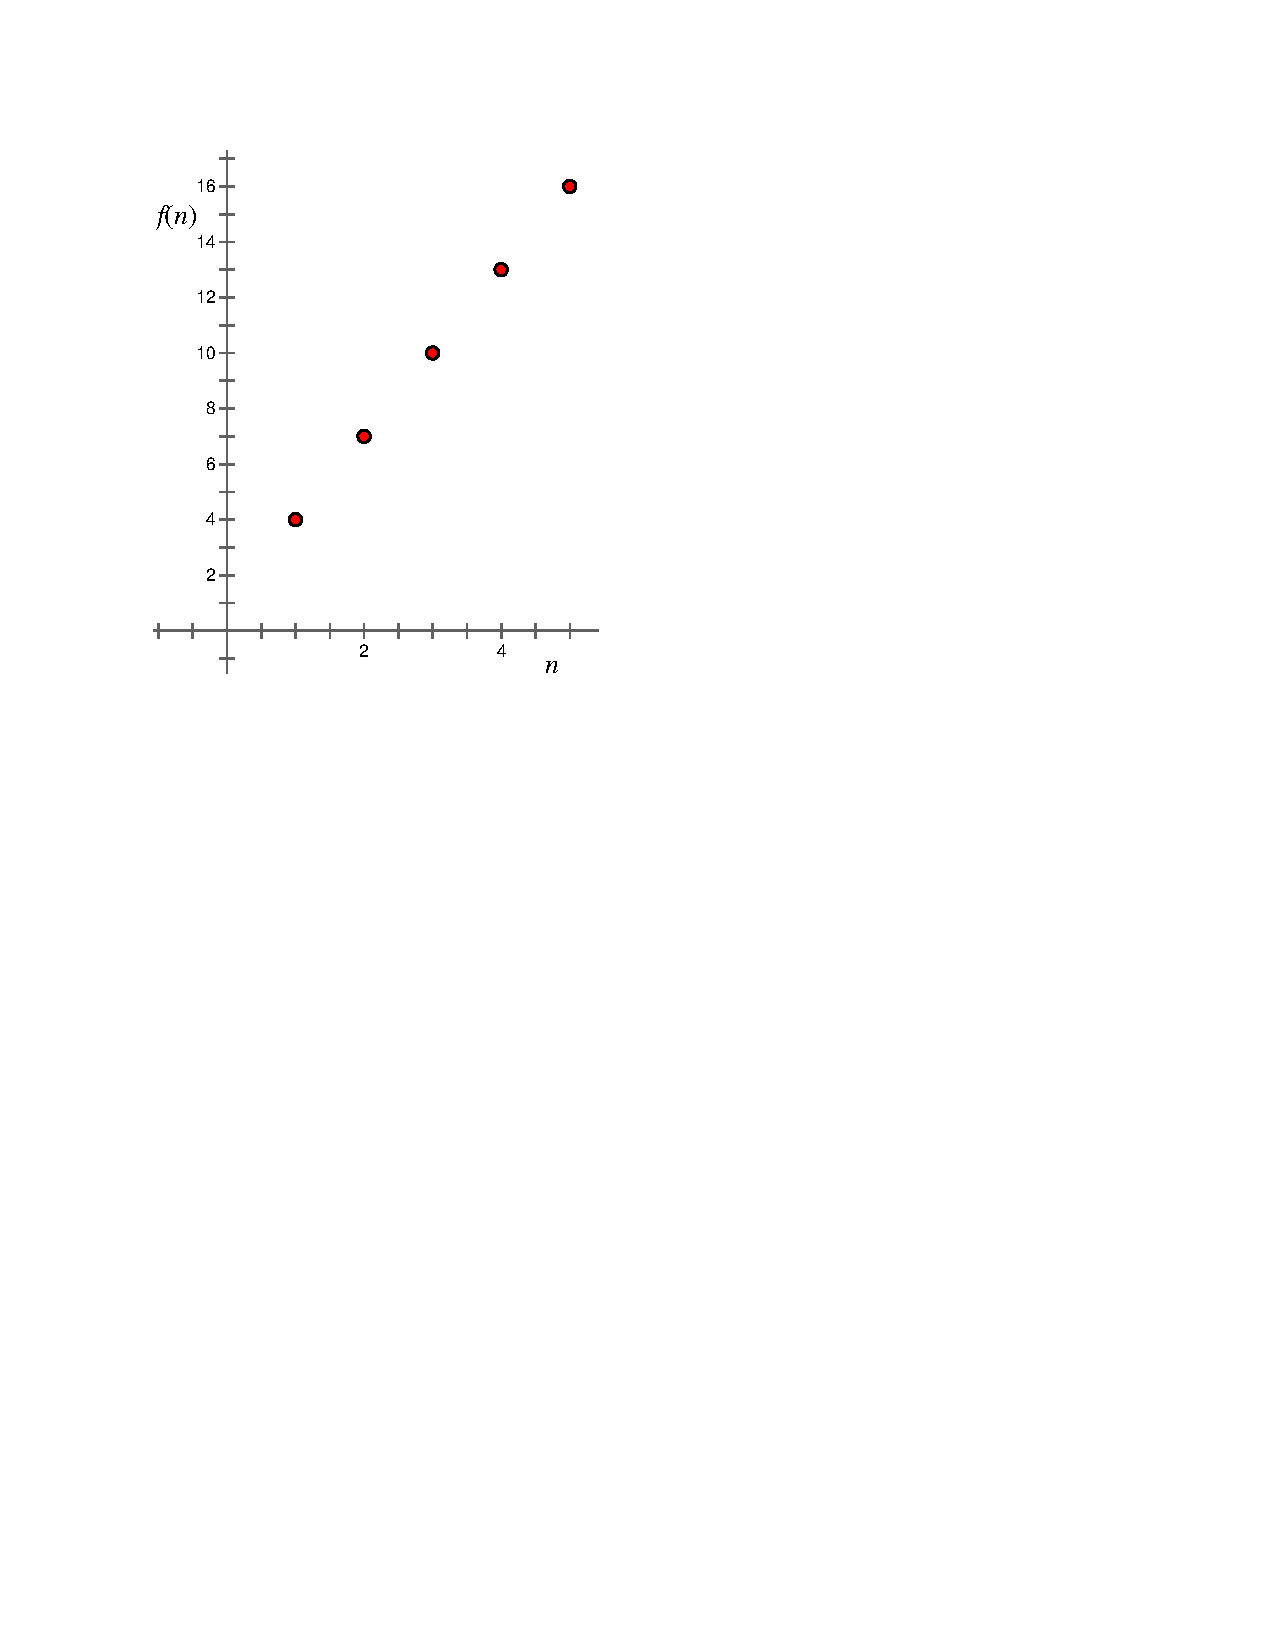
\includegraphics[width=2in]{../graphics/Graph-F2.pdf}} 
of the sequence consists of discrete dots, because the specification does not indicate what happens ``between the dots.''  Connecting the dots requires the assumption that domain values between the dots make sense in some way.  


\begin{question}
In your own words, what does it mean to say that sequences are functions?
\end{question}

\begin{question}
Given that $f(1) = f(2) = 1$, and $f(n+1) = f(n)+f(n-1)$ for integers $n>2$, find $f(6)$.  
\end{question}

\paragraph{Arithmetic and Geometric Sequences.}  An \emph{arithmetic sequence} has is a constant difference between consecutive terms.  A \emph{geometric sequence} has a constant ratio between consecutive terms.  Some sequences, of course, are neither arithmetic nor geometric.\standardhs{F-BF.2}
\begin{question}
For each of the following sequences, decide whether it is arithmetic, geometric, or neither, and explain your reasoning:
\begin{itemize}  
\item $1, 4, 9, 16, 25, \dots$
\item $4, 8, 16, 32, \dots$
\item $2, 4, 6, 8, 2, 4, 6, 8, \dots$
\item $-2, 5, 12, 19, \dots$
\end{itemize}
Can you write both recursive and explicit formulas for each of these sequences?  
\end{question}

Beginning in about grade 8, much of school mathematics is devoted to the study of linear, quadratic, and exponential functions.\standardhs{F-LE.2}  Here we provide only definitions and key questions about these types of functions.  

\begin{itemize}
\item A linear function is of the form $f(x) = ax + b$, where $a$ and $b$ are real numbers and $a\ne 0$.  What do $a$ and $b$ tell you about the linear function?  
\item A quadratic function is of the form $f(x) = ax^2 + bx + c$, where $a$,  $b$, and $c$ are real numbers and $a\ne 0$.  What do $a$, $b$, and $c$ tell you about the function?  Why is it important to specify that $a\ne 0$? 
\item An exponential function is of the form $f(x)=ab^x$, where $a$ and $b$ are real numbers and $b>0$.  What do $a$ and $b$ tell you about the function? 
\end{itemize}

How can you identify these types of functions in tables, graphs, symbols, and contexts?\standardhs{F-IF.4} \standardhs{F-IF.7}  
For example, how can you recognize the slope in the graph of a linear function?  What about in a table, in a symbolic expression, or in a context?  

\begin{question}
An arithmetic sequence is what kind of function?  Explain. 
\end{question}
\begin{question}
A geometric sequence is what kind of function?  Explain.  
\end{question}

\begin{question}
Sometimes quadratic functions are written in the form $f(x) = a(x-h)^2+k$, where $a$, $h$, and $k$ are real numbers and $a\ne 0$.  What do $a$, $k$, and $h$ tell you about the function?  What are the advantages and disadvantages of this form of a quadratic, as compared to the alternative form given above?  
\end{question}

\paragraph{Series.}  A \emph{series} is a sum of consecutive terms from a sequence.  A series with terms that form an arithmetic sequence is called an \emph{arithmetic series}.  

\begin{question}
Find the sum:  $1 + 3 + 5 + \dots + 4999.$  (First explain how you know this is an arithmetic series.)
\end{question}

In mathematics teaching and learning, it is useful to distinguish \emph{problems} from  \emph{excercises}. \emph{Problems} require that you formulate a solution strategy, whereas \emph{exercises} are about using a procedure that you have been taught.\margincomment{Problem solving is an essential part of mathematics.}  Whether a question is a problem or an exercise depends upon the learner.  
\begin{question}
Is the previous question a problem or an exercise for you?  
\end{question}

When analyzing any series, it is often useful to consider the \emph{sequence of partial sums}.  For example, in response to the above question, the sequence of partial sums is as follows:  $$1, \qquad 1 + 3, \qquad 1+ 3+5, \qquad 1+3+5+7, \qquad \dots$$

Sometimes you can see a pattern in the sequence of partial sums.  Making a conjecture about a pattern is a type of inductive reasoning.  Once you notice a pattern, an important next step is showing, deductively, that the pattern \emph{must} continue.  

For arithmetic series, there are several observations that can lead to a general deductive argument for the sum.  For example, consider pairing the first term with the last term, the second term with the second-to-last term, and so on.  What do you notice about the sum of each of these pairs?  And how many such pairs are in the whole series?  Alternatively, consider the average of each of the pairs and how those averages might help determine the sum of the whole series.  An important general technique involves writing the series backward immediately below a forward version and then adding vertically.  

\begin{question}
Use one of these approaches to show that the sum is what it is.  Can you use a picture to illustrate your reasoning?    
\end{question}

\begin{question}
When you consider the sequence of partial sums of an arithmetic series, what kind of function(s) can you get?  Explain.  
\end{question} 

A series with terms that form a geometric sequence is called a \emph{geometric series}.  

\begin{question}
Find the sum:  $\frac{2}{3}+\frac{2}{9}+\dots+\frac{2}{3^{10}}$.  (First explain how you know the series is geometric.)
\end{question}

For the question above, it is not hard to see a pattern in the sequence of partial sums.  In fact, it is reasonable to believe that the pattern holds for any (finite) partial sum of the infinite geometric series $\frac{2}{3}+\frac{2}{9}+\dots$.  But to show that the pattern always holds, we need a general argument.  

For geometric series, the techniques for arithmetic series do not carry over.  Instead, observe that if you multiply the series by the common ratio, the resulting series has most of the same terms as the original series.  Thus, the difference between the two series (i.e., subtract the two) is a short expression that is not hard to work with.  

\begin{question}
Use these ideas to show that the sum is what it is.  Can you use a picture to illustrate this sum?    
\end{question}

\begin{question}
Convert $0.\overline{42}$ to a fraction.  What connections do you see with geometric series?  
\end{question}

\paragraph{Concluding Remarks.}  When studying arithmetic and geometric sequences and series, it is easy to encapsulate common results into compact formulas.  But formulas are easily confused with one another and otherwise misremembered.  Furthermore, general formulas can obscure the ideas.  

\begin{question}
Find the missing terms in the following arithmetic sequence:  
$$\rule[-2pt]{25pt}{.5pt}, \rule[-2pt]{25pt}{.5pt},  2,  \rule[-2pt]{25pt}{.5pt}, \rule[-2pt]{25pt}{.5pt}, 6, \dots$$
Explain your reasoning.  
\end{question}

\begin{question}
Find exact values (not decimal approximations) for the missing terms in the following geometric sequence:  
$$\rule[-2pt]{25pt}{.5pt}, \rule[-2pt]{25pt}{.5pt},  2,  \rule[-2pt]{25pt}{.5pt},  \rule[-2pt]{25pt}{.5pt}, \rule[-2pt]{25pt}{.5pt}, 6, \dots$$
Explain your reasoning.  And describe how this problem and the rules of exponents might be used to explain the connection between radicals and exponents.  
\end{question}

\begin{question}
What key ideas behind arithmetic and geometric sequences did you use in the previous two problems? 
\end{question}

\begin{question}
Explain briefly the key ideas behind finding the sum of an arithmetic series. Then do the same for geometric series.  
\end{question}

\begin{center}
\textbf{With the ideas, you can reconstruct the formulas you need.  And without the ideas, formulas are empty.}  
\end{center}

%\appendix
%
%\renewcommand{\theenumi}{$(\mathrm{\alph{enumi}})$}
%
%\renewcommand{\labelenumi}{\theenumi}
%\chapter{Activities}
%\addtocontents{toc}{\protect\setcounter{tocdepth}{0}}


% \newpage
\section{The Triathlete}\label{A:Triathlete}

\begin{prob} 
On Friday afternoon, just as Laine got off the bus, she realized that she had left her bicycle at school.  In order to have her bicycle at home for the weekend, she decided to run to school and then ride her bike back home.  If she averaged 6 mph running and 12 mph on her bike, what was her average speed for the round trip?  Explain your reasoning. 
\end{prob}

\begin{teachingnote}
A key idea here is that the average speed is independent of the distance.  Here are several ways that students can solve it: 
\begin{itemize}
\item Pick a distance, say 12 miles.  Then running to school will take 2 hours, and biking back home will take 1 hour.  That's a total of 24 miles in 3 hours, or an average of 8 mph.  
\item Let the distance be $d$.  Then running to school will take $\frac{d}{6}$ hours, and biking back home will take $\frac{d}{12}$ hours.  The total distance is $2d$.  So the average rate is 

$$\frac{2d}{\frac{d}{6}+\frac{d}{12}}=\frac{2}{\frac{1}{6}+\frac{1}{12}}=\frac{2}{\frac{3}{12}}=\frac{2}{\frac{1}{4}}=8 \text{ mph}$$
Notice that the $d$ factors out of both the numerator and the denominator (and hence cancels), which shows that the average speed is independent of the distance.  

Notice also that this calculation can be expressed as a different kind of average:  $$\frac{\frac{1}{6}+\frac{1}{12}}{2}=\frac{1}{8}$$
This average is called the \emph{harmonic mean}.  Specifically, 8 is the harmonic mean of 6 and 12 because it is the reciprocal of the average of their reciprocals.  (Math 1165 students do not need to know this language.)
\item Sometimes is helpful to think of speed as ``time per distance,'' which is the reciprocal of ``distance per time.''  In this problem, we can reason that Lanie runs a ``ten-minute mile" as follows:  Her speed of 6 mph would be $\frac{1}{6}$ hour/mile, which is the same as 10 min/mile.  Similarly, she bikes at 5 min/mile.  With this insight, we can cut the distance between home and school into 1-mile pieces and reason that she will take 10 minutes to run each mile and 5 minutes to bike the same mile on the way home.  That would be 15 minutes for both directions (2 miles), for an average speed of 7.5 min/mile, which is the same as 8 mph.  
\item Another way of thinking about these kinds of problems is as weighted averages.  For example, because the distances are the same, Laine will spend twice as much time running (i.e., at half the speed) as she spends on her bike.  Thus, we can weight the 6 mph running speed twice and the 12 mph biking speed just once, as follows:  
$$\textrm{Average speed }= \frac{2\cdot6 + 12}{3} = 8.$$
Notice we divide by 3 because that is the sum of the weights.  The same reasoning can work even when the numbers are more challenging.  
\end{itemize}
\end{teachingnote}

\begin{prob}
On Saturday, Laine completed a workout in which she split the time evenly between running and cycling.  If she again averaged 6 mph running and 12 mph on her bike, what was her average speed for the workout?  Explain your reasoning. 
\end{prob}

\begin{teachingnote}
Here the naive calculations works:  The average speed is the average of the two speeds, so the answer is $\frac{6+12}{2}=9$ mph.  But we should be clear why this works.  Here are two approaches: 
\begin{itemize}
\item Pick a time, say 1 hour, to spend on each activity.  Lanie will run 6 miles in 1 hour and will bike 12 miles in 1 hour.  That will be 18 miles in 2 hours, or an average of 9 mph.  This will work, of course, for every hour of activity, which suggests that the result is independent of time.  
\item Algebra:  Let the $t$ represent the time spent on each activity.  The distance running will be $6t$, the distance biking will be $12t$, and the total time will be $2t$.  So the average speed will be $$\frac{6t+12t}{2t}=\frac{18t}{2t}=9 \text{ mph.}$$  
Notice the common factor of $t$ cancels, which shows that the average speed is independent of the time.  
\end{itemize}
\end{teachingnote}

\begin{prob}
Why was her average speed on Saturday different from her average speed on Friday?  Can you reason, without computation, which average speed should be faster?  
\end{prob}

\begin{teachingnote}
One approach:  When the times are the same, the average will be midway between the two speeds.  When the distances are the same, in contrast, she will spend more time traveling at the slower speed than at the faster speed, so the average will be closer to the slower speed, which implies that the same-distance average is slower than the same-time average.  
\end{teachingnote}

\begin{prob} On Sunday, Laine's workout included swimming.  Assuming that she can swim at an average speed of 2 mph, describe two running-cycling-swimming workouts, one similar to Friday's scenario (same distance) and a second similar to Saturday's (same time).  Compute the average speed for each and explain your reasoning.  
\end{prob}

\begin{teachingnote}
Same distance (a la Friday):  

$$\text{Average speed } = \frac{3d}{\frac{d}{2}+\frac{d}{6}+\frac{d}{12}}=\frac{3}{\frac{1}{2}+\frac{1}{6}+\frac{1}{12}}=\frac{3}{\frac{9}{12}}=\frac{3}{\frac{3}{4}}=4  \text{ mph.}$$

Same time (a la Saturday):  $$\text{Average speed } = \frac{2t+6t+12t}{3t}=\frac{20t}{3t}=6\frac{1}{3} \text{ mph.}$$
\end{teachingnote}

\begin{prob}
Which of the workout scenarios (same distance or same time) most closely resembles an actual triathlon?  Why do you think that is the case?
\end{prob}

\begin{teachingnote}
In actual triathlons, the running distances are much shorter than the biking distances, and the swimming distances are much shorter still.  It would not be reasonable to swim any reasonable biking distance.  So the ``same time'' scenario is closer.  But in reality, the swimming times are quite a bit shorter than the running and biking times.  
\end{teachingnote}

\begin{prob}
After two months of intense training, Laine is able to average $s$ mph swimming, $r$ mph running, and $c$ mph cycling.  Again describe two running-cycling-swimming workouts, one similar to each of the two original scenarios, and compute her average speeds.     
\end{prob}

\begin{teachingnote}
Same distance (a la Friday):  

$$\text{Average speed } = \frac{3d}{\frac{d}{s}+\frac{d}{r}+\frac{d}{c}}=\frac{3}{\frac{1}{s}+\frac{1}{r}+\frac{1}{c}}$$

Same time (a la Saturday):  $$\text{Average speed } = \frac{st+rt+ct}{3t}=\frac{(s+r+c)t}{3t}=\frac{s+r+c}{3}$$
\end{teachingnote}



\end{document}
